%%%--------------------------------%%%
%%% Theory
%%%--------------------------------%%%
\section{Progressive Web Apps}
\label{sec:theorieC}


As of today, devices such as mobile phones and personal computers come with their own app store. Microsoft offers their own Store, Google its Play Store and Apple the App Store. As a user you often find yourself worrying about an app you once saw running on another platform not being available for your platform too (e.g. Apples iOS and Googles Android). \cite[p. 3]{sheppardBeginningProgressiveWeb2017} Not to mention app developers who are in a hurry to make their apps available for all known platforms.

Progressive Web Apps (PWAs) approach these concerns by trying to move away from app stores onto a platform which is available on most devices – the web browser. This means that PWAs are regular web apps at their core but can progressively leave the web browser. For example, PWAs can be installed on the underlaying operating system and be accessed from the app switcher or the taskbar and be executed in full screen mode without the browsers interface being visible. \cite[p. 26]{liebelProgressiveWebApps2019} Further characteristics of PWAs and how exactly a PWA can leave the web browser are granularly described in the following chapter.


\subsection{Characteristics of a Progressive Web App}
\label{sec:theorieCa}


To transform an existing Web App into a PWA or build one from scratch one must implement different criteria’s instead of including a new framework or library. \cite[p. 6]{sheppardBeginningProgressiveWeb2017}
The following eight characteristics represent Mozilla’s (Firefox) ideas of a PWA. Other web browser manufactures such as Microsoft (Edge) or Google (Chrome) for example describe eight or ten respectively within their developer documentations. \cite[p. 90]{liebelProgressiveWebApps2019}\cite{ProgressiveWebApps}

\begin{enumerate} 
	\item  \textbf{Progressive}: The first characteristic defines that a PWA should not exclude the user from using the core functionality but extend the user experience by embracing new features implemented by the web browser manufactures. \cite[p. 100]{liebelProgressiveWebApps2019}\cite[p. 2]{hajianProgressiveWebApps2019}. For example, a web app to check mails should not exclude the user from checking their inbox or sending mails but could provide push notifications to inform about incoming mails. In this example the user is not excluded from using the core functionality of a mail app (checking the inbox and sending mails) and user experience is enhanced by push notifications. To avoid unexpected failures a developer should follow the \textit{Feature Detection} principle which says an application should not blindly use a non-standardized feature before checking its existence. \cite[p. 101]{liebelProgressiveWebApps2019}

	\item \textbf{Network Independent}: Using a regular web app on the go can be a problem, especially in regions with little to no mobile reception or no stable Wi-Fi being around. Thus, the dynamic content of a web app does not load within a tolerable timeframe or a user is inhibited to perform actions like sending a mail. \cite[p. 106]{liebelProgressiveWebApps2019} On these grounds a technology called \textit{Service Worker} has been established and implemented by many browser manufactures. In short, a service worker is a script that is able to listen to the network traffic caused by a PWA and therefor is able to cache possible answers fetched from a server and serve them to the web app when no stable network connection is available or do background syncing by running code even when the web app isn’t in use. For more information about the service worker see chapter \ref{sec:theorieCc} (p. \pageref{sec:theorieCc}). \cite[p. 43]{sheppardBeginningProgressiveWeb2017}

	\item \textbf{Safe}: As mentioned in the previous paragraph, service workers can run code independently from the PWA. To avoid harmful service workers from running malicious code, browser manufactures expect PWAs to be served by a trusted host over a secure connection. To be more precisely, over an HTTPS connection. \cite[p. 24]{sheppardBeginningProgressiveWeb2017} \textit{HTTPS} stands for Hypertext Transfer Protocol Secure and is based on \textit{TLS} (Transport Layer Security). Once the host has obtained a digital certificate for its domain, this certificate is being transferred to the client where it can be verified by the web browser. On success an HTTPS connection can be established and every upcoming network traffic will be encrypted. \cite[pp. 112-113]{liebelProgressiveWebApps2019}

	\item \textbf{Re-engageable}: A feature which native apps are using for a while now are push notifications. Push notifications are a common way to inform users about the newest events such as a new mail in the user’s inbox. Thanks to the Push API that is implemented on top of the service worker, just like native apps, PWAs can keep the users engaged by sending notifications as it can be seen in figure \ref{fig:pwa_reengageable}. \cite[p. 201]{hajianProgressiveWebApps2019}

\begin{figure}[htbp] 
	\centering
	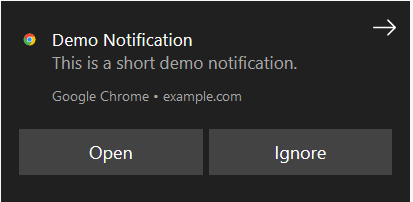
\includegraphics[width=0.4\textwidth]{Assets/chapter_pwa/demonotification.PNG}
	\caption{Push notification to keep users engaged}
	\label{fig:pwa_reengageable}
\end{figure}

	\item \textbf{Responsive}: This characteristic specifies that the PWA render its user interface corresponding to the devices used to access it. This is necessary as the available space and input method can change from device to device. The screen of a phone on average is way smaller than the screen of a notebook. Furthermore, using fingers to interact with a phone is less precise than using a mouse on a notebook. \cite[pp. 115-116]{liebelProgressiveWebApps2019} In figure \ref{fig:pwa_responsive} for example one can see how the content and navigation arranges differently on each device. Due less space the navigation bar on the mobile version (extract on the right side) is completely collapsed and can be accessed by clicking the so-called burger-like icon while on the desktop version the whole navigation bar is visible.

\begin{figure}[htbp] 
	\centering
	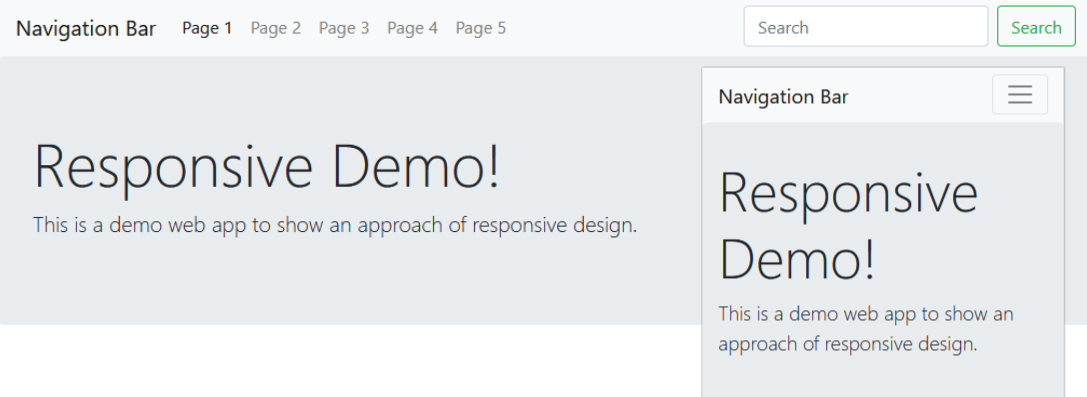
\includegraphics[width=0.8\textwidth]{Assets/chapter_pwa/responsive-overall.jpg}
	\caption{Responsive design}
	\label{fig:pwa_responsive}
\end{figure}

	\item \textbf{Discoverable}: As PWAs are not a new framework or library but regular web apps at their core, there needs to be method to distinguish between a PWA and a regular web app. This is necessary for web browsers to provide additional features to PWAs such as an option to install (see next paragraph). To make a PWA discoverable a “Web Manifest” file (see chapter \ref{sec:theorieCb}, p. \pageref{sec:theorieCb}), which contains information like the name of the PWA, needs to be provided. \cite[p. 118]{liebelProgressiveWebApps2019}

	\item \textbf{Installable}: To take things even further, besides offline functionality, a PWA should be installable to the user’s device. In detail, a user should be able to install the PWA from within the web browser to the underlaying operating system like Android or iOS. From this point on the user can launch the PWA directly from the devices home screen like it is shown in chapter \ref{sec:theorieCb} (p. \pageref{sec:theorieCb}). Different browser manufactures expect different requirements to be fulfilled before they provide an option to install. Mozilla’s Firefox for example expect that the PWA is network independent, safe and discoverable. \cite{HowMakePWAs}

	\item \textbf{Linkable}: The last characteristic implies that a PWA is referable by a \textit{URL} (Uniform Resource Locator, e.g. “www.example.com”) instead of being in the need to be installed via any app store. Ideally, the URL should also point to different views of a PWA like a profile page of a specific person. Hence, the current view can be easily shared between users. As PWAs are being run by a web browser, which need an URL to access the web app in first place, this characteristic, in its fundamentals, does not require any further attentiveness by the developer. \cite[pp. 126-127]{liebelProgressiveWebApps2019}
\end{enumerate}

\subsection{Web Manifest}
\label{sec:theorieCb}

The web manifest is a \textit{JSON} (JavaScript Object Notation) file. Its primary task is to make a PWA discoverable and installable (see chapter \ref{sec:theorieCa}, p. \pageref{sec:theorieCa}) by providing descriptive information, like a short app name and paths to icons, about the PWA. 
The following listing shows a minimal web manifest:

\begin{center}
	\begin{minipage}{\textwidth}
		\lstinputlisting[
		style = fancy,
		language = json,
		label = alg:pwa_wm,
		caption = Example Web Manifest
		]{manifest.json}
	\end{minipage}
\end{center}

The \texttt{(short-)name} represent the name of the PWA which is used on the app switcher or home screen, depending on how much space is available. \texttt{icons} contains various file path to app icons with different sizes which are used in different scenarios like the app switcher, home screen or the apps splash screen. For each use case the most appropriate size is chosen automatically. \texttt{start\_url} defines the entry point of the PWA, \texttt{display} holds information about how the PWA will be displayed once it is installed (e.g. \texttt{standalone} for no web browser elements) and finally \texttt{theme}- and \texttt{background\_color} which determine the primary color of the user interface and the background color of the splash screen respectively. \cite{HowMakePWAs}

Figure \ref{fig:pwa_webmanifest} shows the effects of this web manifest on an example PWA. On the left one can see the use of the icon and name field in Googles Chrome “Add to Home Screen” prompt. In the middle the short name is used due the given space. Once the PWA is launched, like on the right, the standalone display mode is used which hides all elements of the web browser. 

\begin{figure}[htbp] 
	\centering
	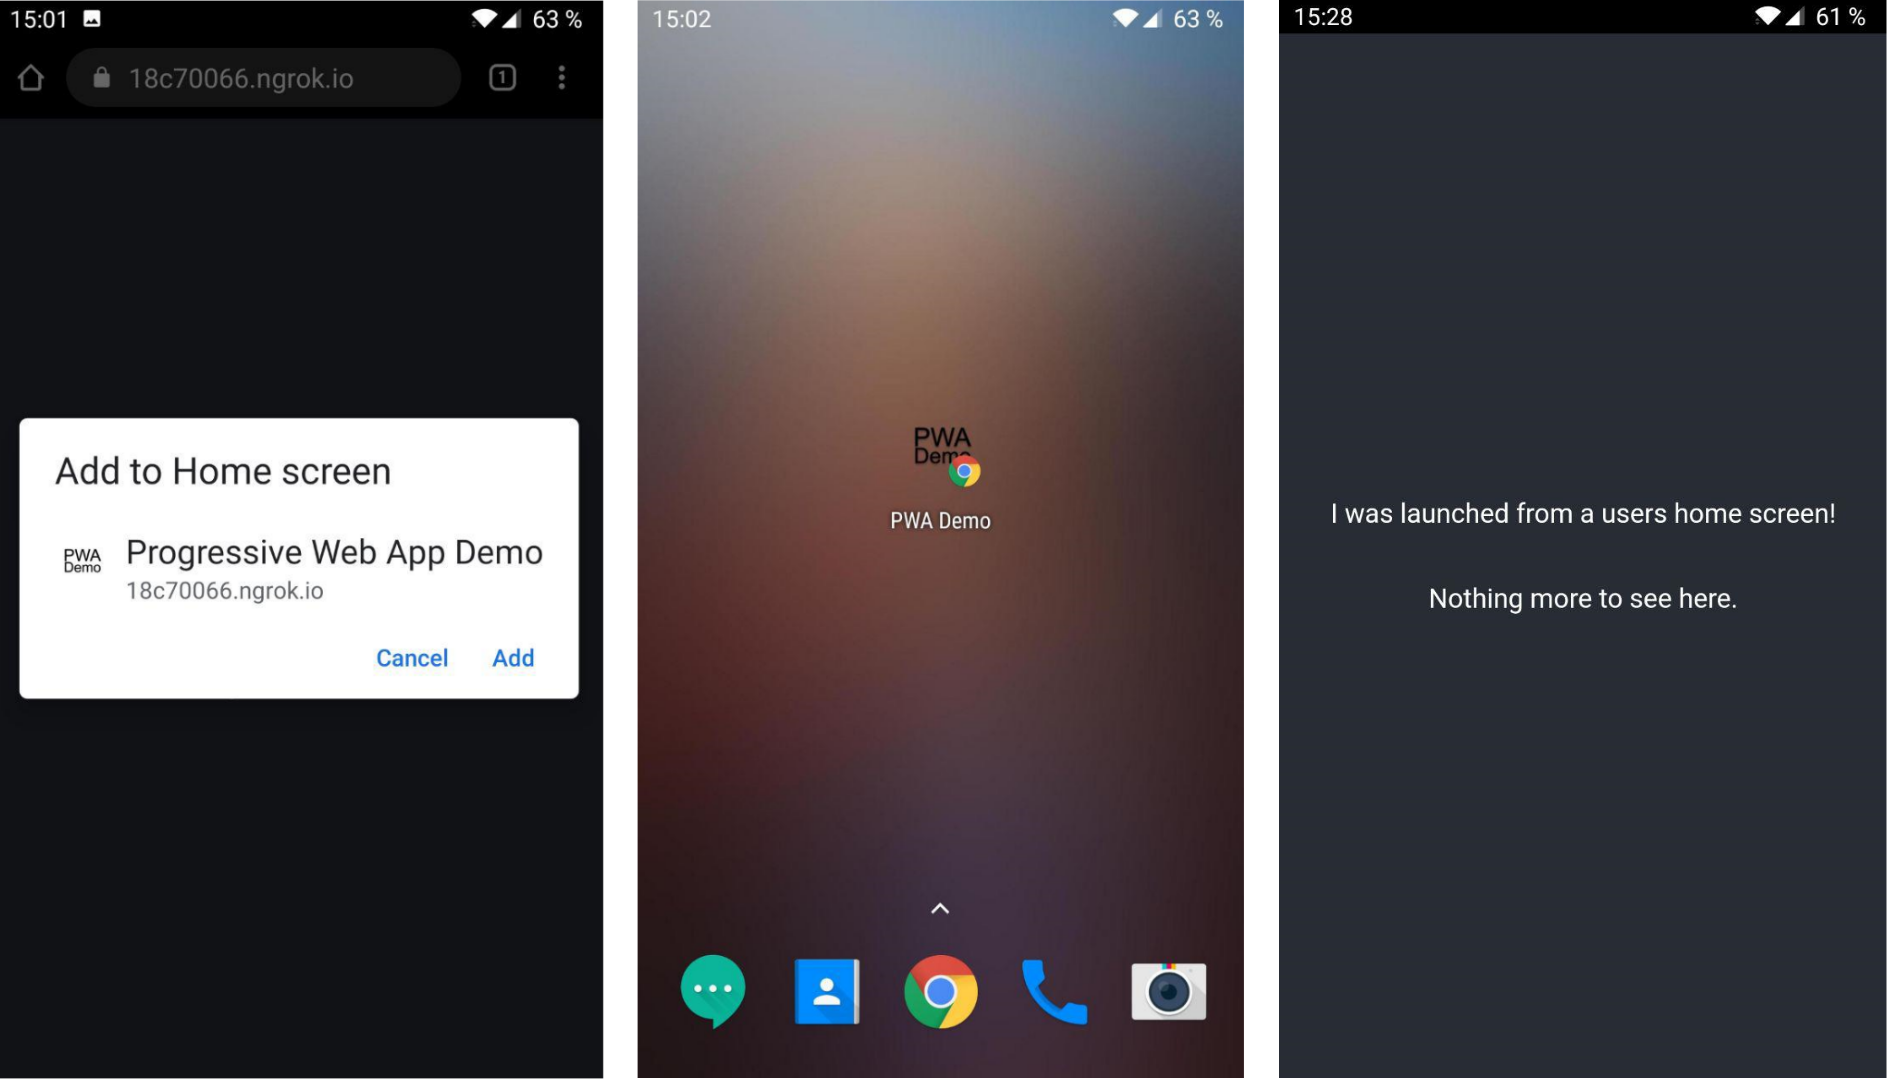
\includegraphics[width=0.8\textwidth]{Assets/chapter_pwa/manifest_demo.png}
	\caption{Outcome of the web manifest}
	\label{fig:pwa_webmanifest}
\end{figure}

\subsection{Service Worker}
\label{sec:theorieCc}

A service workers, a in JavaScript written script which runs in the context of the web browser, primary purpose, as mentioned in chapter \ref{sec:theorieCa}(p. \pageref{sec:theorieCa}), is to cache content and provide it to the PWA whenever a slow or no connection to the Internet exists. Background syncing as well as sending push notifications can also be realized with a service worker. To achieve this, a service worker has three specific traits: being \textit{controller}, \textit{interceptor} and a \textit{proxy}. 

After being registered by the web browser, which means that a HTTPS connection is established and it is request by the PWAs source code, it has full control to all in- and outgoing network traffic, hence the trait of a controller. Interceptor means that the service worker can manipulate and inspect the network traffic and proxy as the service worker is able to decide if the outgoing traffic should be redirected to the requested resource or completely avoid any outgoing traffic by answering with data it stored in a cache previously. The latter is the exact reason why a service worker is indispensable for the Network Independent characteristic (chapter \ref{sec:theorieCb}, p. \pageref{sec:theorieCb}) of a PWA.

The upcoming listing demonstrate how a service worker can manipulate and proxy outgoing network traffic. Before, lets assume that a cache called \texttt{pwa-demo} was already created by the service worker.

\begin{center}
	\begin{minipage}{\textwidth}
		\lstinputlisting[
		style = fancy,
		language = ES6,
		label = alg:pwa_sw,
		caption = Cache First Service Worker
		]{sw.js}
	\end{minipage}
\end{center}

In the first line one can see the service worker is referencing itself and adds an event listener for all fetch-events (requesting data from outside of the web browsers context). The event listener gets passed the fetch \texttt{event} as its second argument on which it calls the \texttt{respondsWith} method. Within that method, it opens the cache called \texttt{pwa-demo} in line two to then check if the requested event matches the data stored in the cache in line three. If it does match, it then directly returns the data back to the PWA. Otherwise it executes the right part of the conditional OR expression \texttt{||} and calls the \texttt{fetch} method to get the data from the requested resource. \cite[p. 60]{liebelProgressiveWebApps2019}

This strategy is called \textit{Cache First} as the service worker will look in the cache before requesting resources outside of the browser’s context. Once cached, the data will available much faster and offline but if the resource change its content, the service worker will still return the old, cached version. On the other side the \textit{Network First} strategy exists that will always fetch data when a connection to the resource (e.g. the Internet) can be established. Thus, the user will always receive the newest content and has a slightly older version available when being offline. On the downside, if the connection is slow the content may take a while to be fetched. Therefore, the \textit{Cache and Network} strategy combines both, the Cache- and Network-First, strategies. To bridge the time of fetching new content, the user is presented the cached content until the result is available and then be presented by refreshing the user interface. These are just a few but popular strategies and each has their own scenarios where they work best. \cite[pp. 109-111]{hajianProgressiveWebApps2019}

\subsection{Compatibility}
\label{sec:theorieCd}


As with every new specification introduced it takes some time until every manufacturer has fully implemented it in their products. In this chapter a short overview of what web browsers, in terms of PWAs, are currently capable of is given. The following figures are taken  of a site called www.CanIUse.com (17/10/2019) which shows to what grade a web browser version supports a  specification. Red means no support, dark green fully supported and light green supported to a specific grade.

In figure \ref{pwa_comptaibility_webmanifest} one can see the web browser compatibility of the web manifest for richer offline experiences like being installable.

\begin{figure}[htbp] 
	\centering
	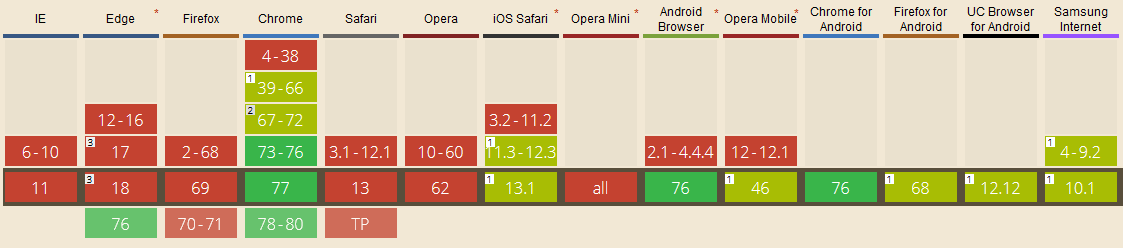
\includegraphics[width=0.9\textwidth]{Assets/chapter_pwa/webmanifestsupport.PNG}
	\caption{Compatibility of the web manifest}
	\label{fig:pwa_comptaibility_webmanifest}
\end{figure}


The web manifest is currently not widely supported on the desktop versions of many browsers. Currently only Googles Chrome fully supports it, in return though, most major, except Opera Mini, mobile browsers at least partly support the web manifest. 

Figure \ref{fig:pwa_comptaibility_serviceworker} shows the web browsers support for the service worker which primary goal is the offline functionality. Regardless of desktop or mobile platform, it is currently supported by every major web browser except the Internet Explorer and Opera Mini.

\begin{figure}[htbp] 
	\centering
	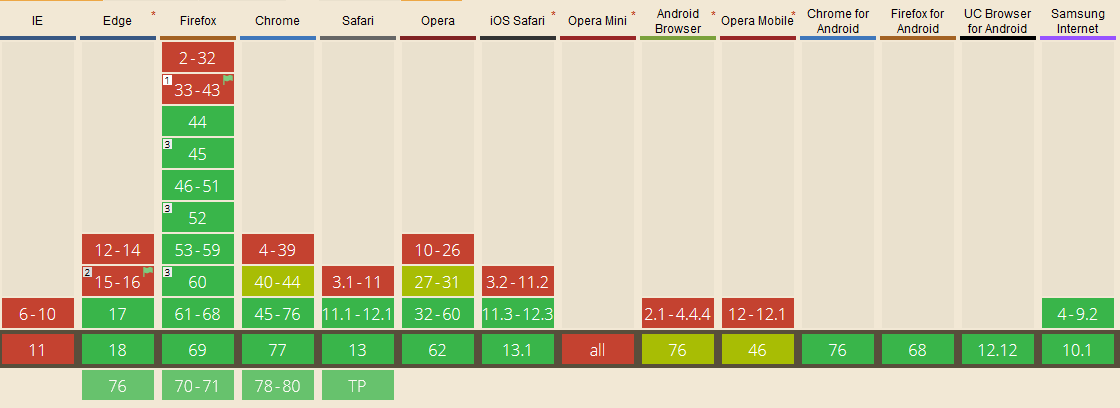
\includegraphics[width=0.9\textwidth]{Assets/chapter_pwa/serviceworkersupport.PNG}
	\caption{Compatibility of the service worker}
	\label{fig:pwa_comptaibility_serviceworker}
\end{figure}

If the PWA should use push notifications to inform its users about new occurrences and fulfill the re-engageable characteristic (see chapter \ref{sec:theorieCa}, p. \pageref{sec:theorieCa}) it can use the Push API which is another specification that needs to be implemented by the web browsers manufacturer.

\begin{figure}[htbp] 
	\centering
	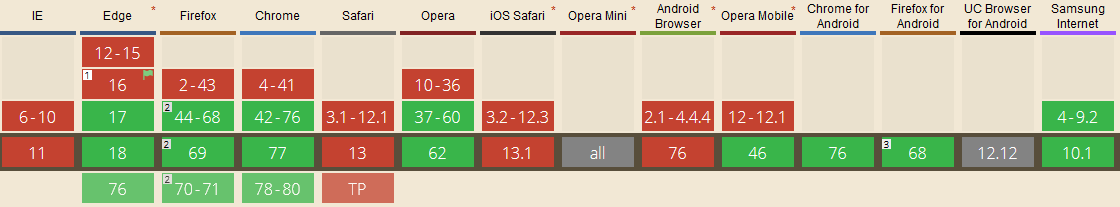
\includegraphics[width=0.9\textwidth]{Assets/chapter_pwa/pushapisupport.PNG}
	\caption{Compatibility of the Push API}
	\label{fig:pwa_comptaibility_pushapi}
\end{figure}

As seen in figure \ref{fig:pwa_comptaibility_pushapi}, most manufactures have implemented this feature, Apple falls behind with their desktop and mobile web browser Safari as well as Microsoft’s Internet Explorer.

Thinking back upon the first characteristic of a PWA, being progressive, a non-supported feature (e.g. the web manifest in Mozilla's Firefox) won’t lock the user out of the app as all these specifications should only enhance the user experience and not lock the user out from using the core functionality of a web app.